\documentclass[12pt]{article}
\usepackage{hyperref}
\usepackage[warn]{mathtext}
\usepackage[T2A]{fontenc}
\usepackage[utf8]{inputenc}
\usepackage[russian]{babel}
\usepackage{cite}
\usepackage{amsfonts}
\usepackage{lineno}
\usepackage{subfig}
\usepackage{graphicx}
\usepackage{xcolor}
\usepackage{bm}
\usepackage{graphicx}
\usepackage{amssymb}
\usepackage{hyperref}
\usepackage[left=2cm,right=2cm,top=2cm,bottom=2cm]{geometry}

\DeclareGraphicsExtensions{.png,.jpg}
\date{14 сентября 2021 г.}
\author{Карцев Вадим}
\title{Лабораторная работа 2.1

Опыт Франка-Герца}

\begin{document}

\maketitle

\textbf{Цель работы:} измерение энергии первого уровня атомов гелия в динамическом и статическом режимах.

\textbf{В работе используются:} серийная лампа ионизационного манометра ЛМ-2, стабилизированный источник питания
Б7-4, микроамперметр, вольтметр, осцилограф C1-83.

\section{Теоретическая справка}
  Опыт Франка-Герца доказывает существование дискретных уровней энергии атома.

  В опыте используется трехэлектродная лампа, наполненная разреженным
  одноатомным газом.

  \begin {figure}[h!]
    \begin{minipage}[h]{0.49\linewidth}
        \center{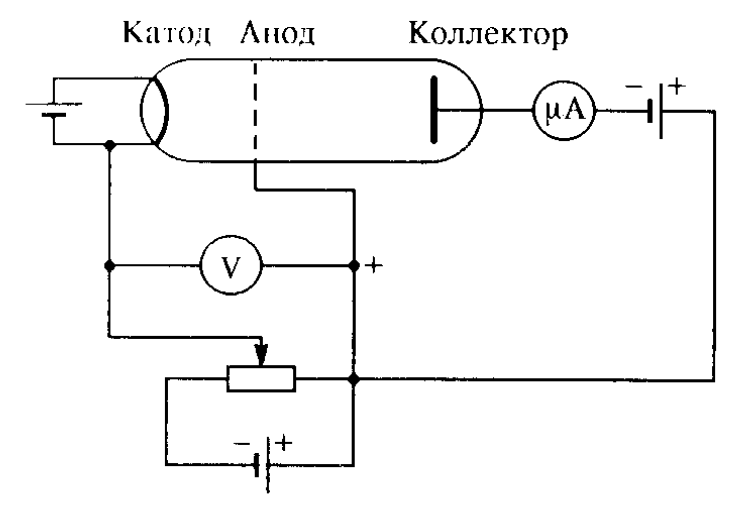
\includegraphics[width = 9cm]{ustanovka.png}}\\
        Рис 1. Схема установки
    \end{minipage}
    \begin{minipage}[h]{0.49\linewidth}
        \center{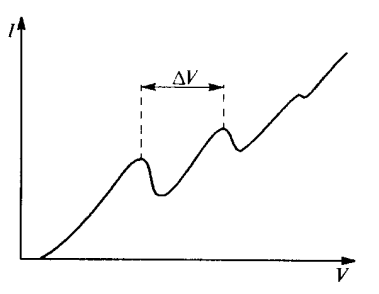
\includegraphics[width = 7cm]{scheme_plot.png}}\\
        Рис 2. Схематическая зависимость тока на коллекторе от разницы потенциалов между анодом и катодом
    \end{minipage}
    \label {fig:image1}
  \end {figure}

  Увеличивая разницу потенциалов между анодом и катодом мы увеличиваем энергия электронов.
  Пока энергии недостаточно для перевода атомов в возбужденное состояние, соударения будут практически
  упругими, т.к. масса электронов мала по сравнению с массой атомов. При дальнейшем увеличении энергии
  электронов начинает хватать для возбуждения или ионизации атомов газа и часть электронов теряет свою энергию
  при соударениях. Таким электронам не хватает энергии преодолеть задерживающее напряжение между анодом и
  коллектором и наблюдается резкое падение тока на последнем.

\section{Получение вольт-амперной характеристики $I_к = f(V_a)$ на экране осцилографа C1-83}

  Рассмотрим полученные осциллограммы

  \begin {figure}[h!]
    \begin{minipage}[h]{0.33\linewidth}
        \center{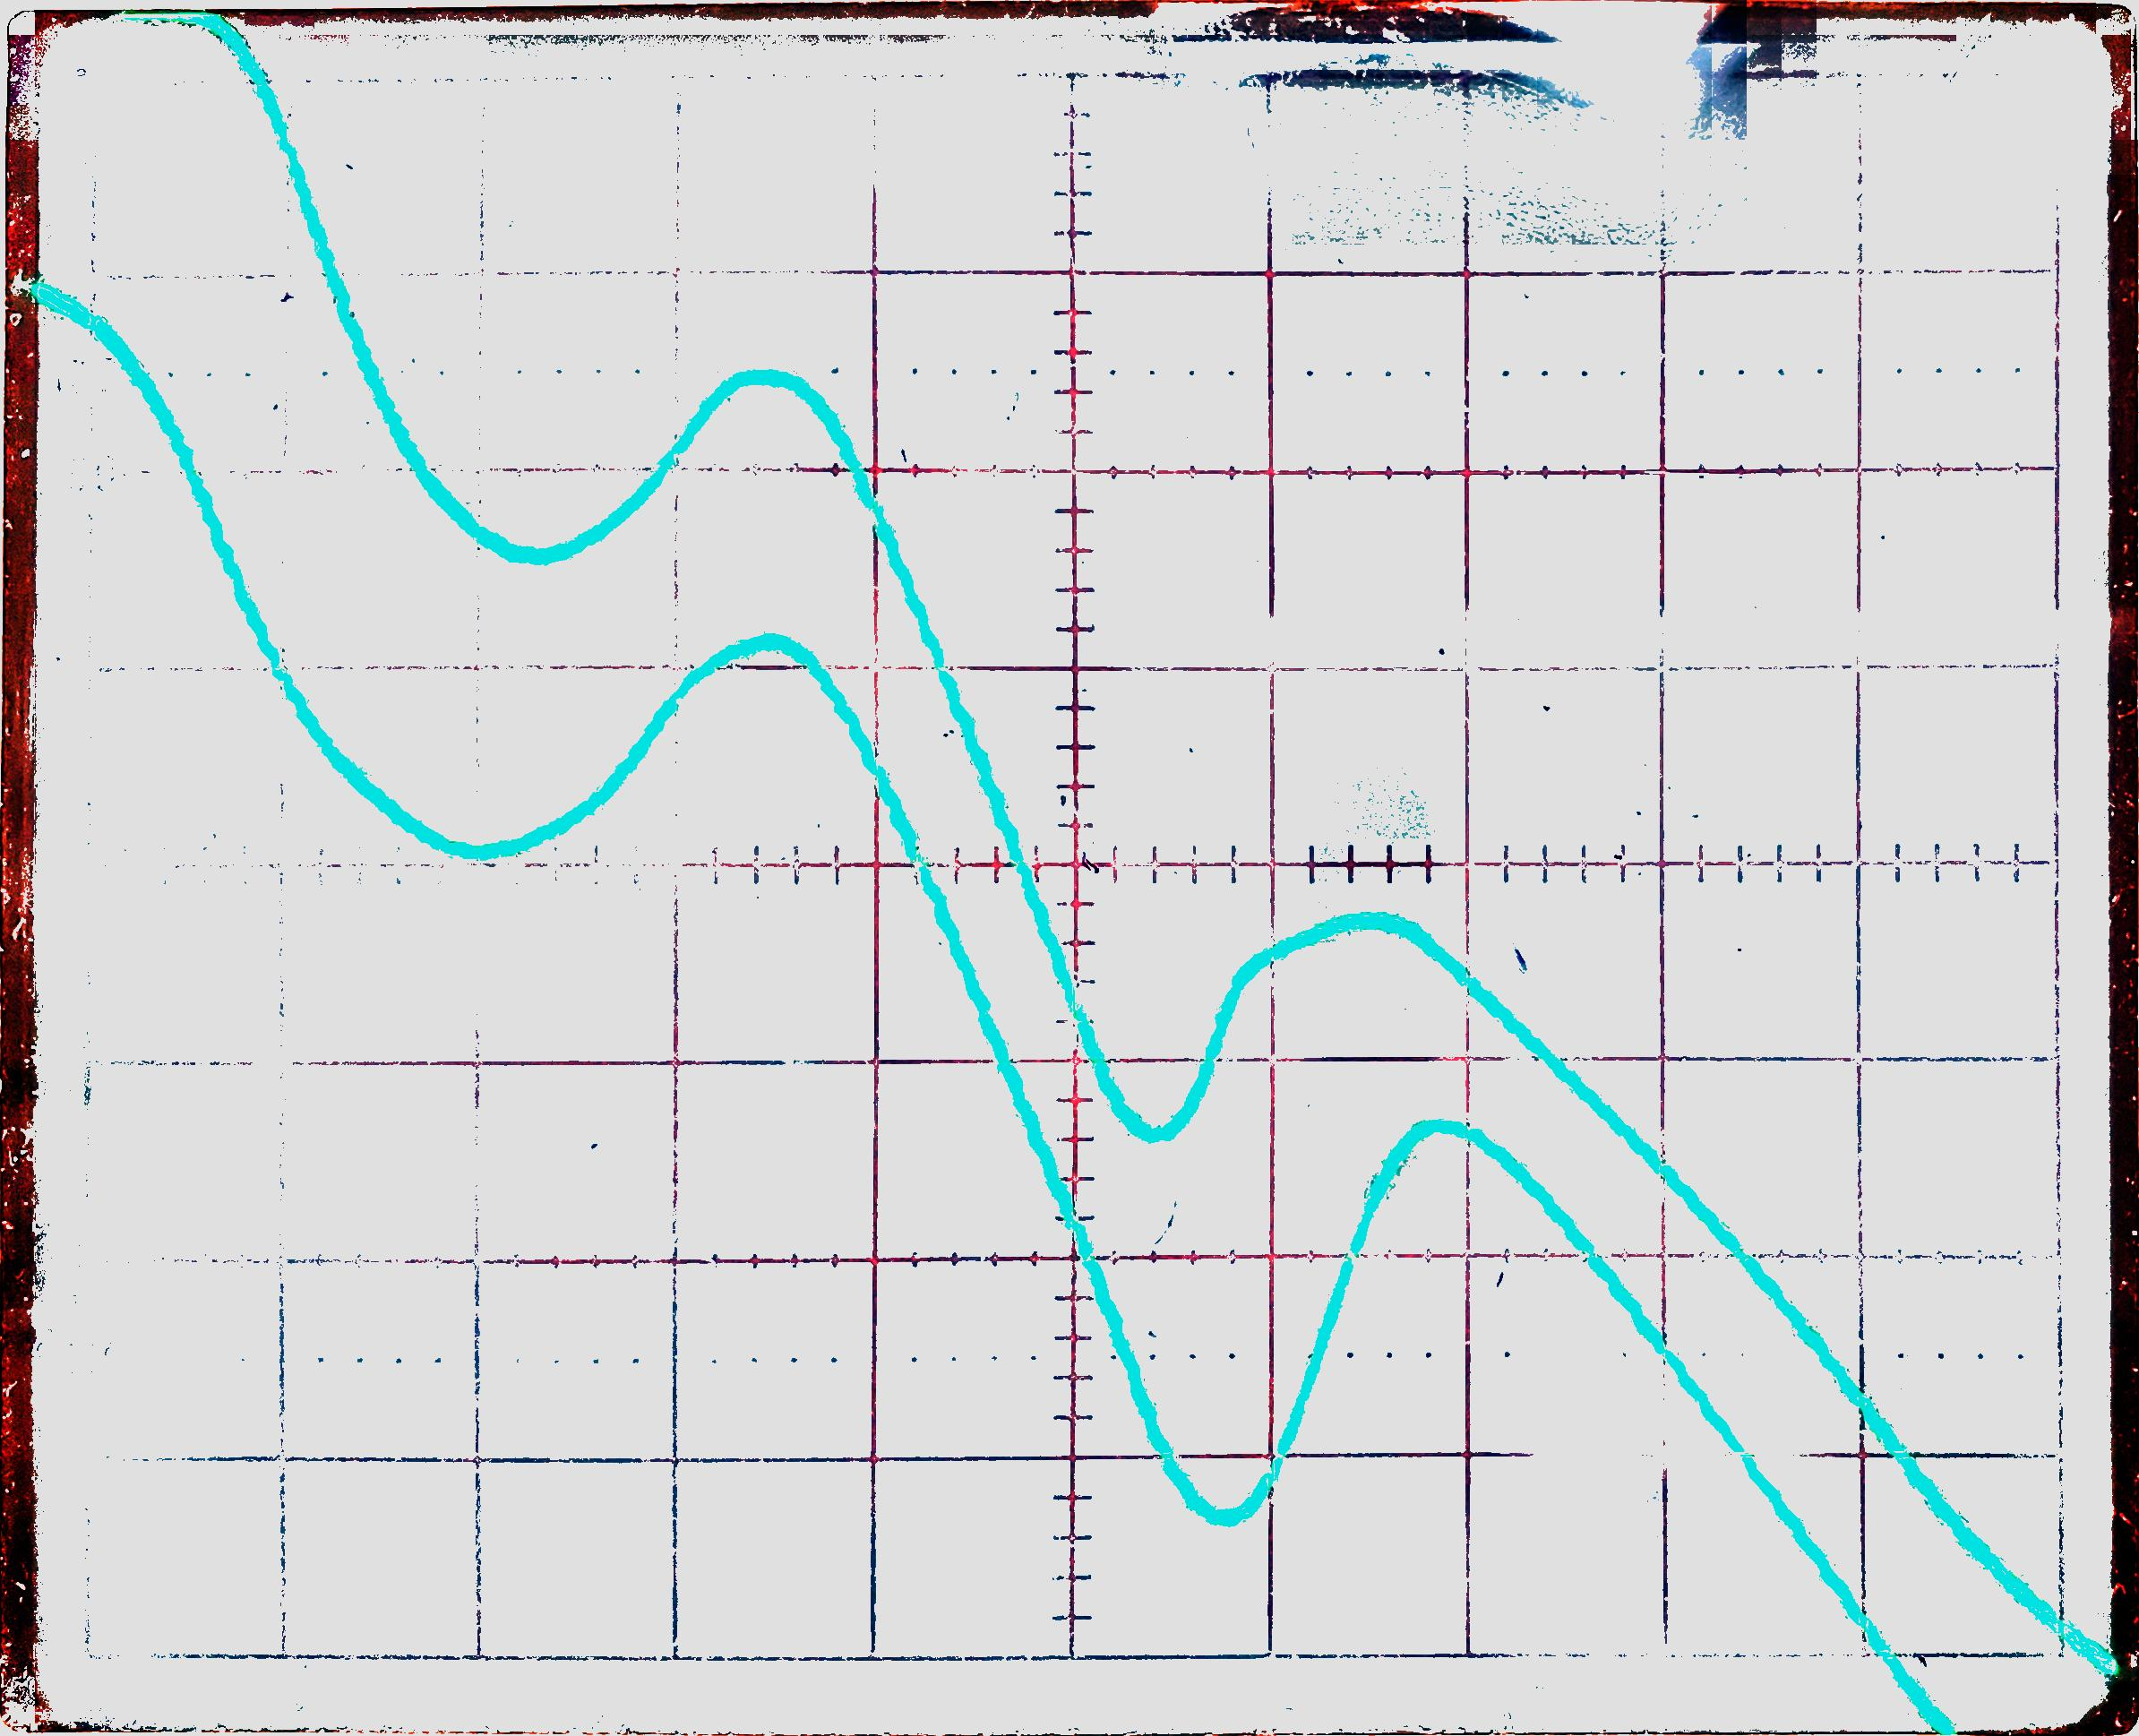
\includegraphics[width = 5.8cm]{oscillogram4V.jpg}}\\
        Рис 3. $V_2 = 4 В$
    \end{minipage}
    \begin{minipage}[h]{0.33\linewidth}
        \center{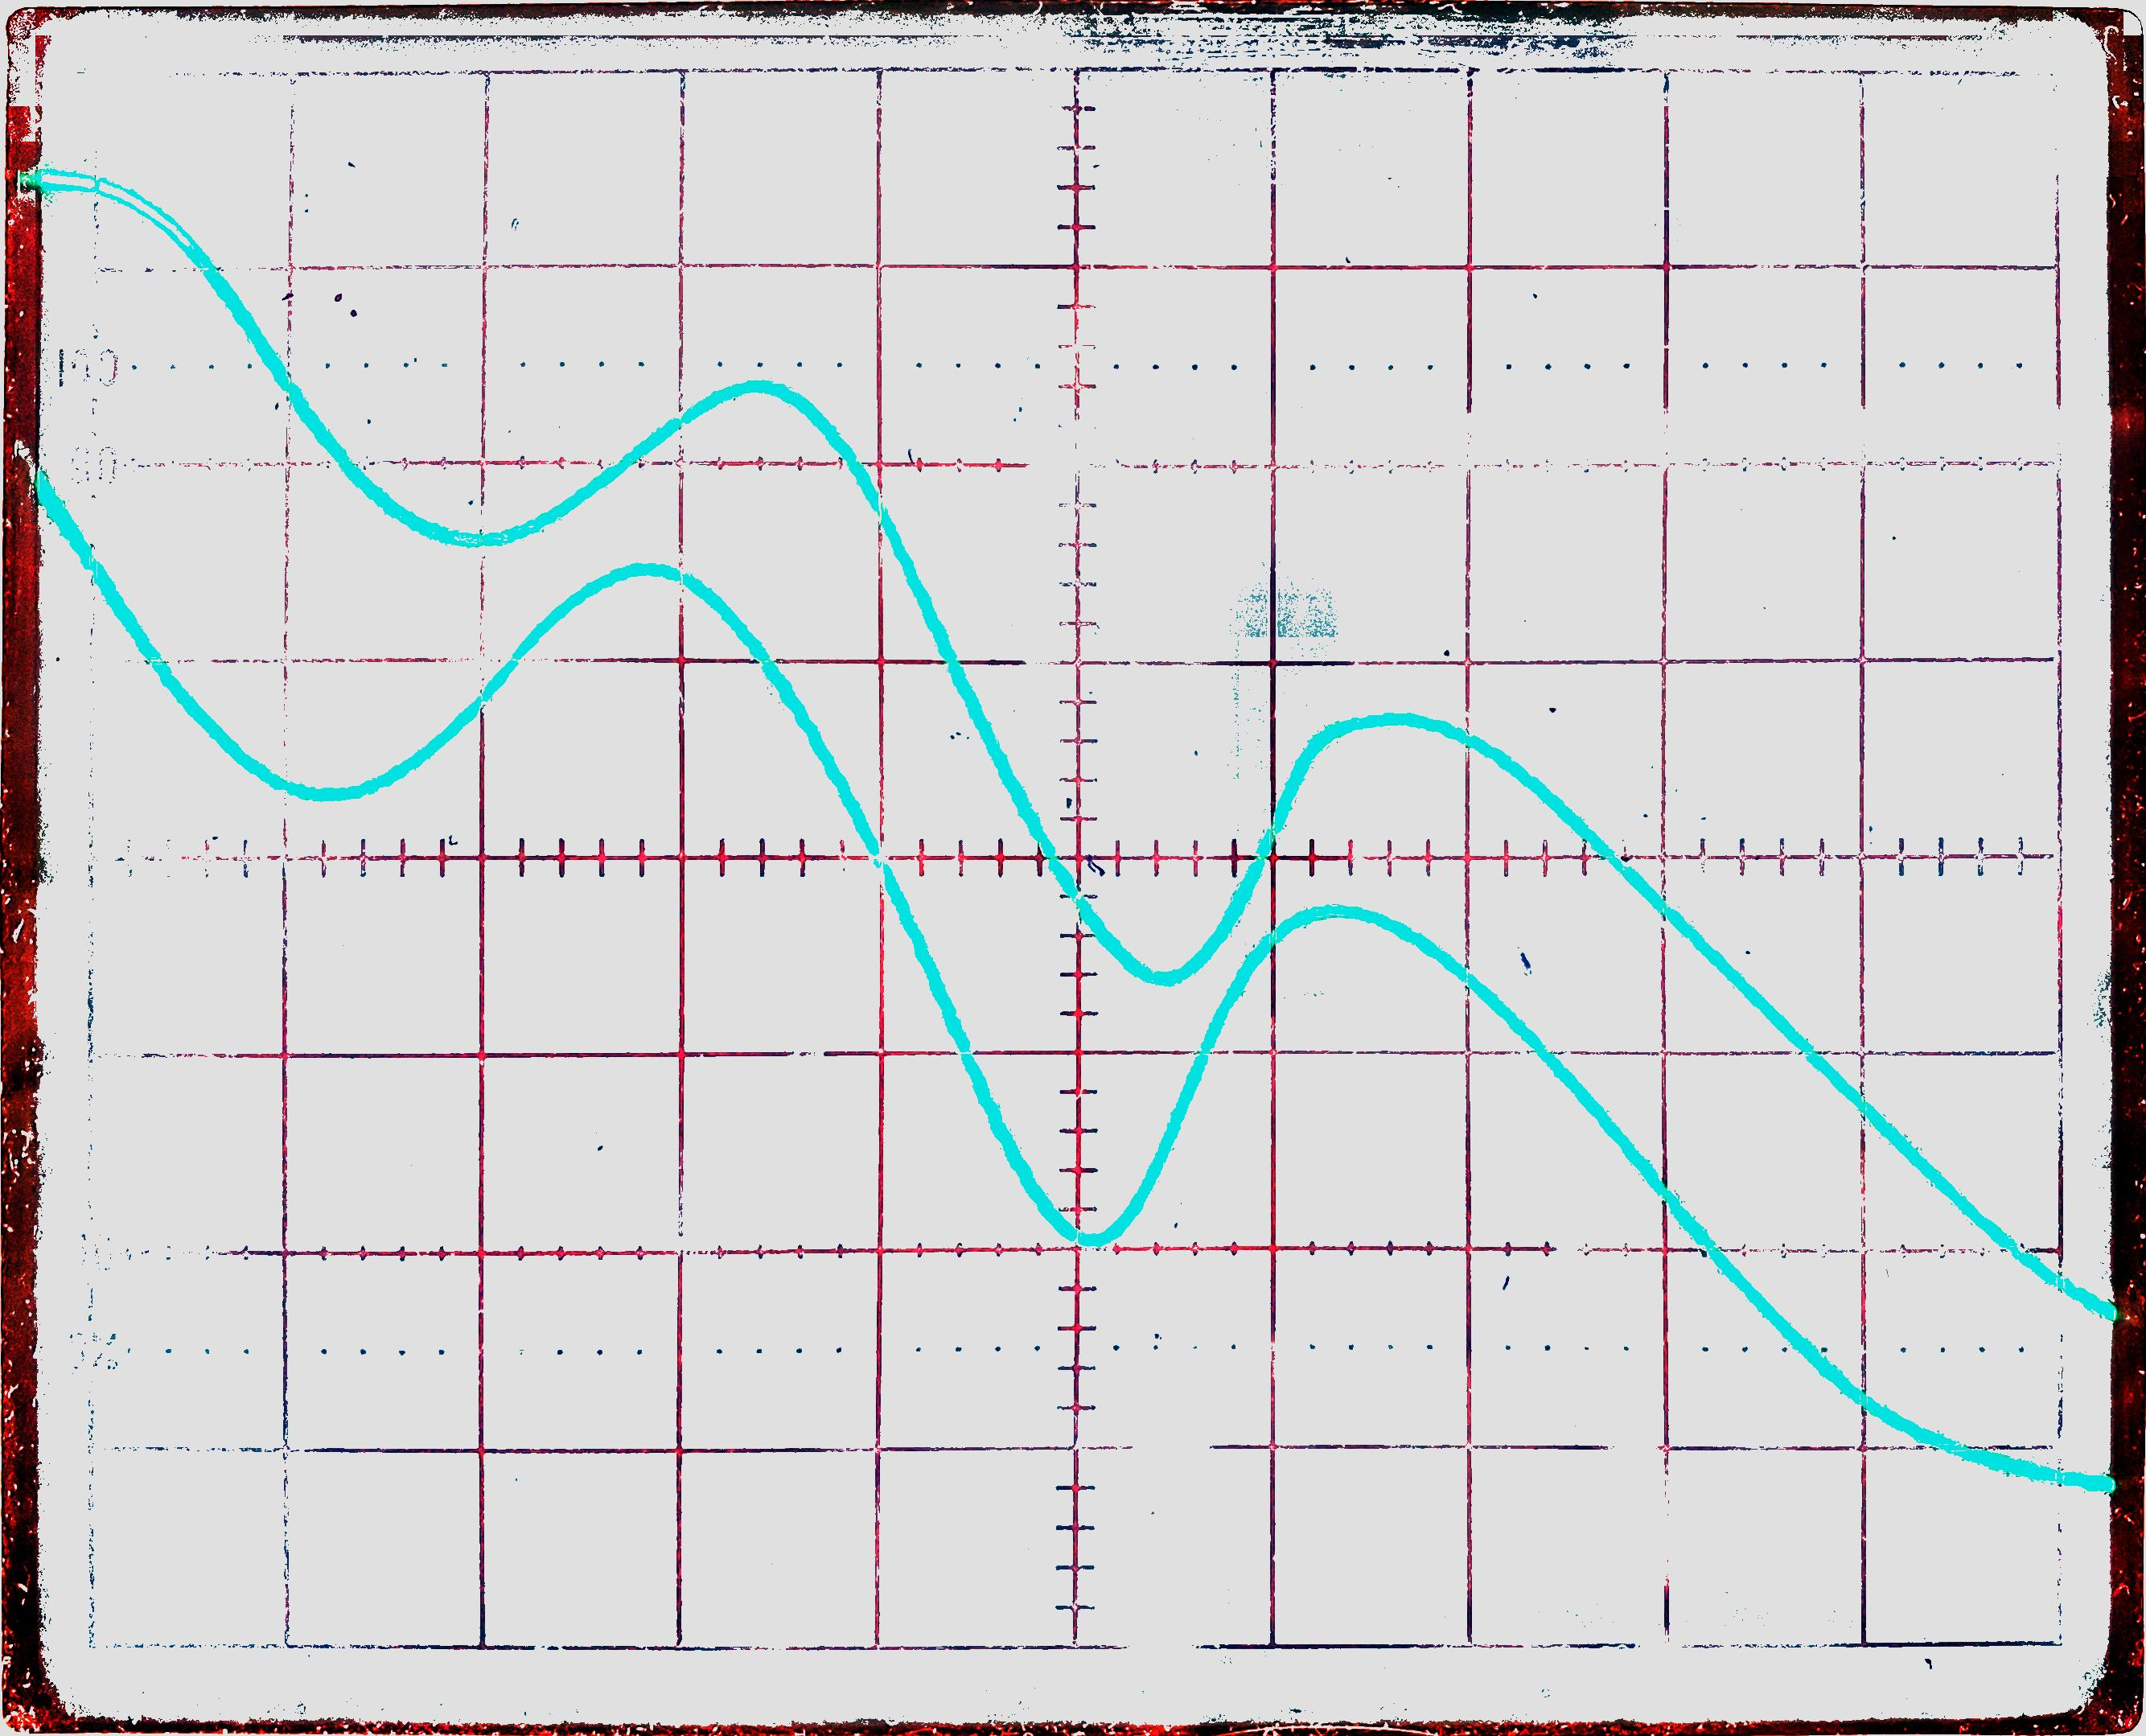
\includegraphics[width = 5.8cm]{oscillogram6V.jpg}}\\
        Рис 4. $V_2 = 6 В$
    \end{minipage}
    \begin{minipage}[h]{0.33\linewidth}
        \center{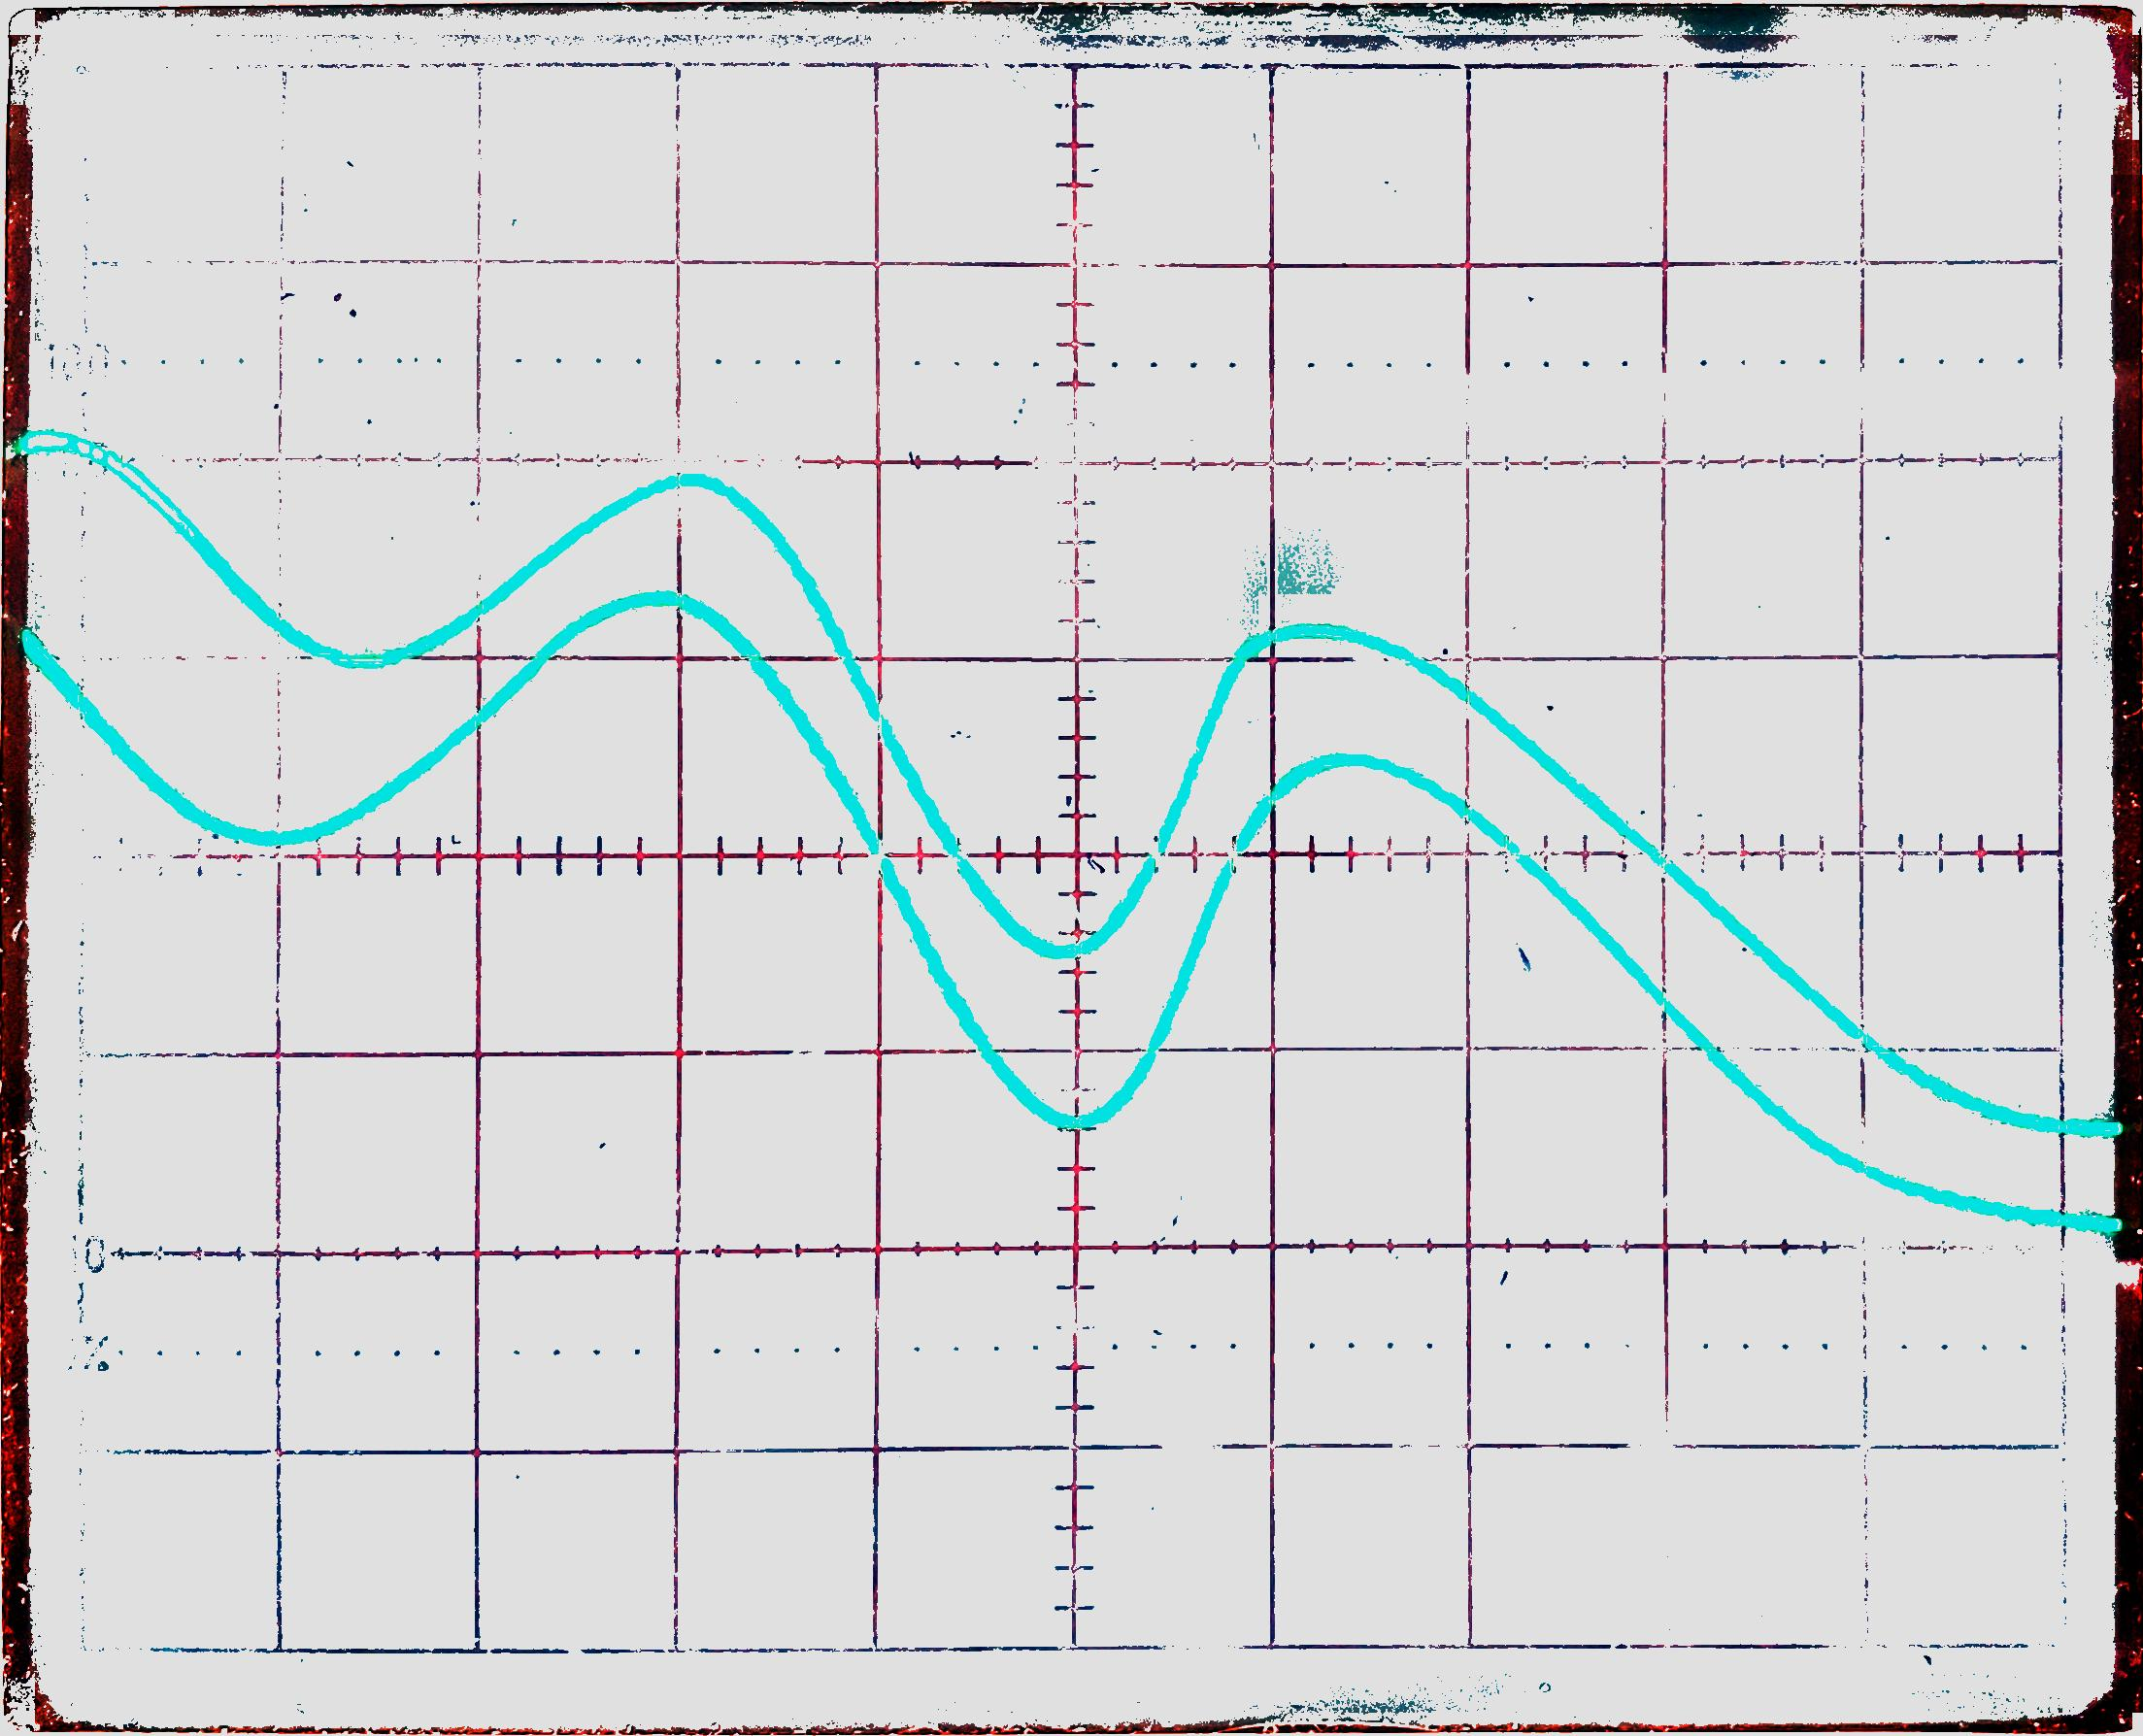
\includegraphics[width = 5.8cm]{oscillogram8V.jpg}}\\
        Рис 5. $V_2 = 8 В$
    \end{minipage}
    \label {fig:image1}
  \end {figure}

  Очевидно, на оцсиллограммах видны прямой и обратный ход. В первом случае напряжение повышается и видно, что ток
  на коллекторе растет с падениями, а во втором случае ток понижается со скачками. Все измерения на осцилографе
  проводились с разверткой $X = 5 В/дел$. Измерим расстояния между максимумами и минимумами в вольтах.

  \begin{figure}[h!]
    \center{Табл 1. Зависимость энергии возбуждения от напряжения торможения}
    \center{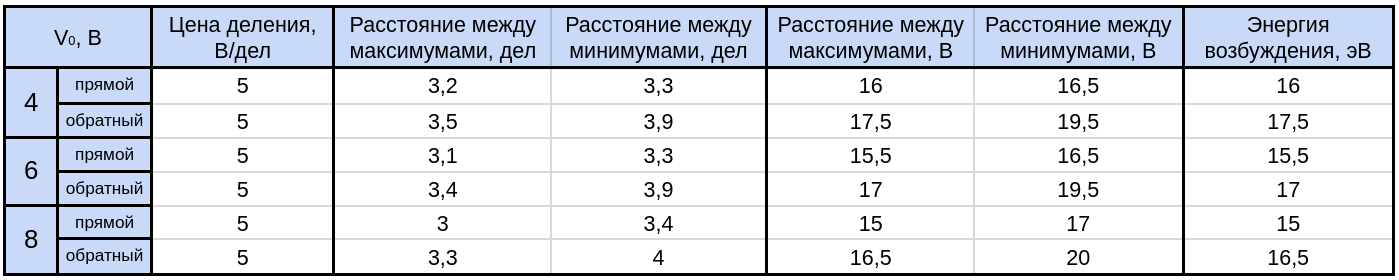
\includegraphics[width = 17.5cm]{table1.png}}
  \end{figure}

  Как видно из таблицы, энергия возбуждения атома гелия будет $E_{возб} = (16.25 \pm 0.94) эВ$, а относительная
  погрешность ее измерения $\varepsilon = 5.76\%$

  \newpage

\section{Получение вольт-амперной характеристики $I_к = f(V_a)$ в статическом режиме измерений}

  \begin{figure}[h]
    \begin{minipage}[h]{0.52\linewidth}
      \center{Табл 2. Зависимость тока коллектора от напряжения на катоде}
      \center{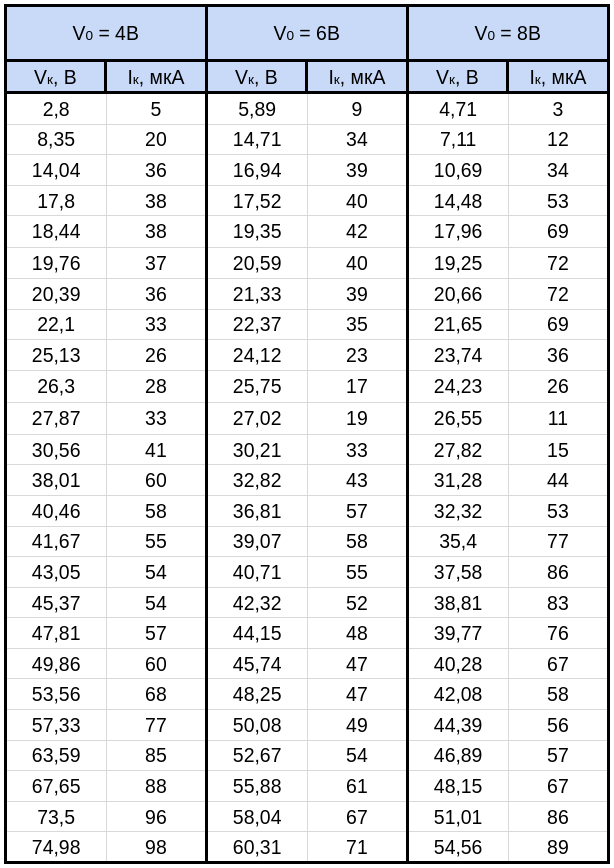
\includegraphics[width=1\linewidth]{table2.png}} \\
    \end{minipage}
    \hfill
    \begin{minipage}[h]{0.47\linewidth}
      \begin{minipage}[h]{1\linewidth}
        \center{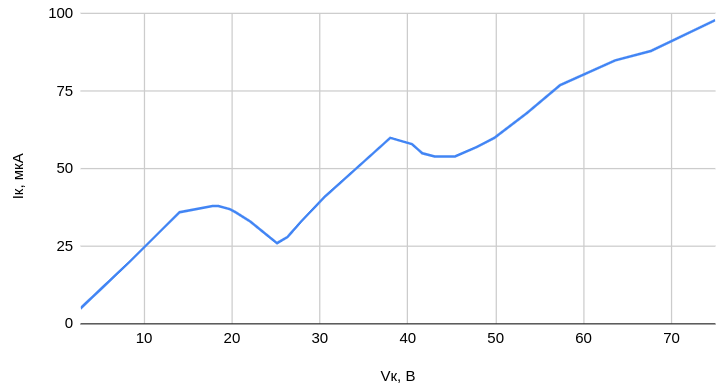
\includegraphics[width=1\linewidth]{plot4V.png}} \\
        Рис 6. $V_0 = 4 В$
      \end{minipage}
      \vfill
      \begin{minipage}[h]{1\linewidth}
        \center{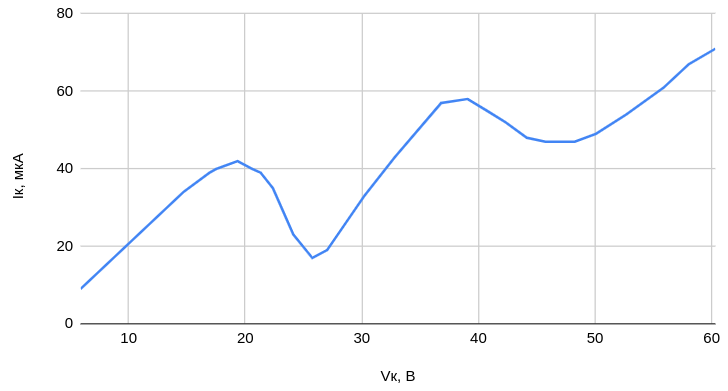
\includegraphics[width=1\linewidth]{plot6V.png}} \\
        Рис 7. $V_0 = 6 В$
      \end{minipage}
      \vfill
      \begin{minipage}[h]{1\linewidth}
        \center{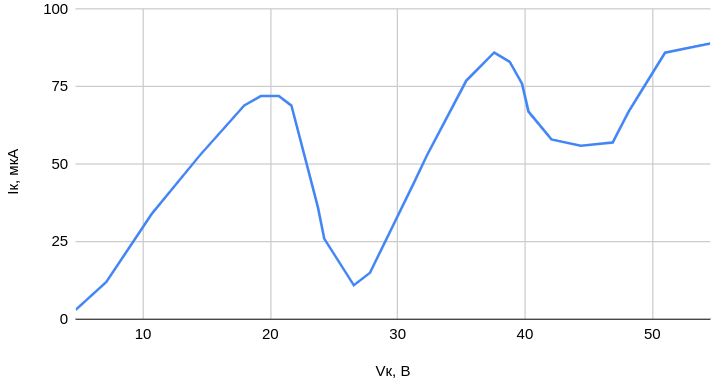
\includegraphics[width=1\linewidth]{plot8V.png}} \\
        Рис 8. $V_0 = 8 В$
      \end{minipage}
    \end{minipage}
    \label {fig:image3}
  \end{figure}

  Из графиков 6, 7 и 8 выясним расстояние между максимумами тока для рассчета энергии возбуждения атома гелия.
  Максимумы выписаны в таблице ниже.

  \begin{figure}[h!]
    \center{Табл 3. Максимумы тока и энергии возбуждения}
    \center{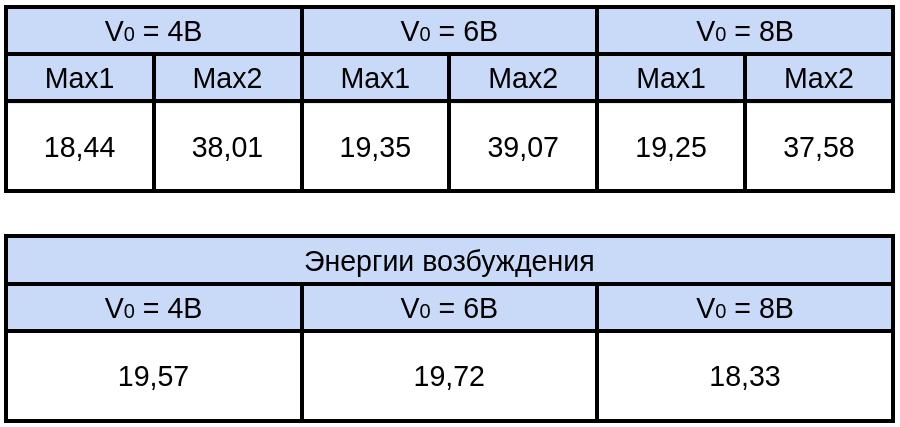
\includegraphics[width = 7.5cm]{table3.png}}
  \end{figure}

  Рассчитаем энергию возбуждения атома гелия и ее погрешность в соответствии с данной таблицей. Легко понять, что
  основной вклад в погрешность вносит нерегулярность измерений, так как приборная погрешность значительно меньше, чем
  минимальное расстояние между измерениями. Таким образом, будем считать погрешность по следующей формуле:

  $$
    \sigma_E = \sqrt{\frac{\sum\limits_{i = 1}^n \left(E_i - \overline{E}\right)}{n - 1}}
  $$

  В нашем случае погрешность $\sigma_E = 0.76$ эВ, а сама энергия первого уровня $E = (19.21 \pm 0.76)$ эВ.
  Относительная погрешность составляет $\varepsilon = 3.96 \%$

\section{Вывод}

  Мы вычислили энергию первого уровня для атомов одноатомного гелия двумя различными способами - динамическим и
  статическим. В первом случае мы получили большую погрешность, что, вероятно, объясняется наличием прямого и
  обратного хода. Кроме того, при увеличении количества точек в статическом методе можно добиться большей точности.
  Расхождения результатов двух вариантов измерения незначительны и по большей части объясняются временем осциляции
  системы, так как в первом случае мы повышаем и понижаем напряжение с большой частотой, что может заметно
  влиять на точность представления результатов, в то время как во втором случае мы дожидаемся полного успокоения
  системы. Табличное значение для энергии первого уровоня атома гелия составляет $24.59$ эВ, что не сильно
  отличается от полученных в ходе эксперимента данных.




\end{document}
